\subsubsection{Autoregression}
\label{subsubsection:processing:ar_modelling}

Even though, differencing and normalization successfully remove some autocorrelations, autoregressive patterns can remain which can be accounted for by autoregressive models. In contrast to their most popular application (e.g. \citet{Ruiz2012CorrelatingActivity}), autoregressive models are not used for forecasting purposes. They are simple linear models with unrealistic constraints and thereby far exceeded by machine learning models \cite{Hsu2016BridgingEconomists}. Nevertheless, they are able to model the linear autoregression of time series which shall be filtered out before cross-correlating time series. If a temporal variable reveals autoregression, a value within this time series can be described by a function of its past values plus an error term $\epsilon$ which is also known as residual. If such autoregression is present for two correlated time series, the calculated correlation coefficient is found to be invalid. Instead, a suitable autoregressive model shall be applied and correlation analysis conducted on the residuals because they are assumed to be free from linear autoregression.

% "Regression models for prediction are often useful even when the assumptions are moderately violated, although they may not perform optimally. However, in many applications, especially with small effects or questions of causality based on observational data, regression methods can give misleading results.[2][3]" (https://en.wikipedia.org/wiki/Regression_analysis)

% History of Time Series Analysis, Types of interventions (omitted vars.), etc. --> https://autobox.com/cms/index.php/afs-university/intro-to-forecasting/doc_download/1-the-autobox-advantage

\paragraph{ARMA}
To remove autoregressive patterns in the mean of the process, an autoregressive-moving-average (ARMA) model is applied \cite{Dionisio2004MutualSeries}. It assumes a temporal observation to be linear combination of the $p$ lagged values and the $q$ lagged error terms from the same stationary and univariate time series \eqref{formula:ar_model}. The remaining value, in the following residual, which cannot be modelled by these terms is called the error term and is assumed to be i.i.d. It should not reveal any significant autocorrelation if an appropriate ARMA model was selected and therefore is valuable for further correlation analysis avoiding spurious correlation \cite{Yule1926WhyTime-Series}. A common approach for determining the hyper parameters, known as Box-Jenkins method \cite{Box1970TimeControl}, uses the autocorrelation function (ACF) and partial autocorrelation function (PACF) \cite{Franke2010StatisticsMarkets}. The ACF describes the correlation of an observation with lag values. The PACF has the same focus but uses a statistically adjusted correlation that is not accounted for by intermediate lags. For the model identification, the number of significant correlation lags from the PACF determines $p$ while the number from the ACF determines $q$. The resulting model is denoted as ARMA(p, q).

% https://machinelearningmastery.com/gentle-introduction-autocorrelation-partial-autocorrelation/
% https://ncss-wpengine.netdna-ssl.com/wp-content/themes/ncss/pdf/Procedures/NCSS/The_Box-Jenkins_Method.pdf
% https://www.academia.edu/2099523/Time_series_analysis_forecasting_and_control
% https://machinelearningmastery.com/gentle-introduction-box-jenkins-method-time-series-forecasting/

\begin{align}
    \returnt{i}{t} &= \sum \limits_{j=1}^{p} a_j \returnt{i}{t-j} + \sum \limits_{j=1}^{q} b_j \epsilon_{t-i} + \epsilon_t  \label{formula:ar_model} \\ \eqname{ARMA Model}
\end{align}

The intraday return at $t$ is regressed by $p$ lagged values $\returnt{i}{t-p}, ..., \returnt{i}{t-1}$ and $q$ lagged error terms $\epsilon_{t-q}, ..., \epsilon_{t-1}$. In order to do so, the model coefficients $a_1, ..., a_p$ and $b_1, ..., b_q$ are fitted with OLS. $\epsilon$ denotes the residual representing the part of $\returnt{i}{t}$ which can not be described by autoregression and therefore is considered to be free of autocorrelation. In the following, the model residual is denoted with $\returnt{i}{t}$. It also involves those stock returns for which no autoregressive modelling was required.

\begin{figure}[!ht]
    \centering
    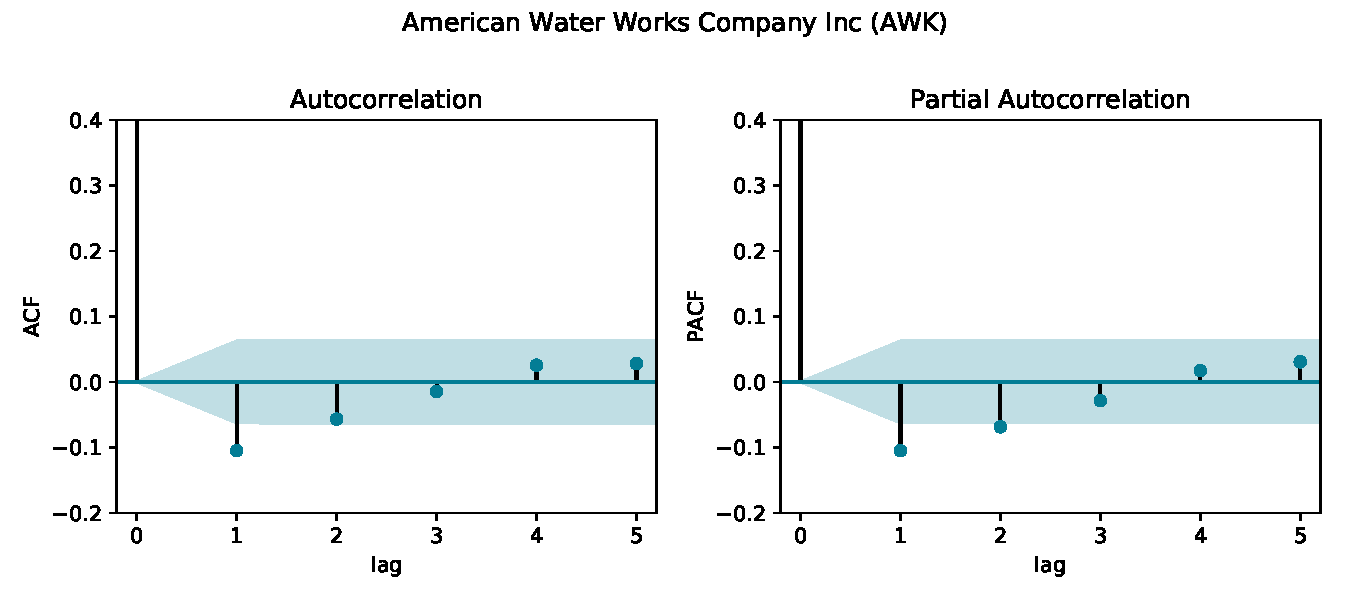
\includegraphics[width=\textwidth]{figures/regression/acf-awk-normed.pdf}
    \caption{ACF and PACF plots for the preprocessed stock returns for company \emph{American Water Works Company Inc}. The x-axis shows the lag and the y-axis shows the correlation coefficient (Pearson's $r$). The colored area around zero represents the 0.95 confidence interval of no significant correlation. All values out of this range can be assumed to be correlated. The autocorrelation of a zero lag will always be one, so the plots are adjusted to not fully show this dispensable data point but put more focus on the following lags.}
    \label{fig:acf_pacf_awk_normed}
\end{figure}

For 385 stocks there was no autocorrelation observable so the ARMA model was not applied on this data. To show an example how lags are determined and how the modelling reduces autocorrelation, the ACF and PACF are plotted in Figure~\ref{fig:acf_pacf_awk_normed} for an example company. The ACF shows significance for one lag while the PACF even shows significance for two lags, so an ARMA(2, 1) model will be applied.

\begin{figure}[!ht]
    \centering
    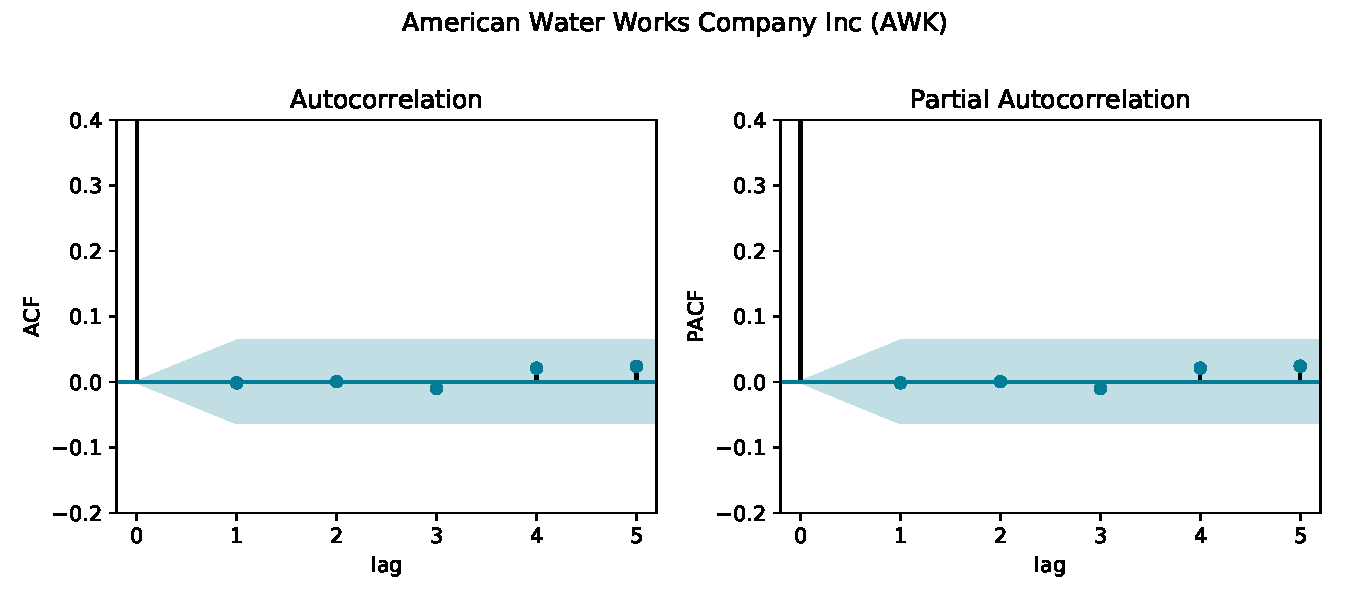
\includegraphics[width=\textwidth]{figures/regression/acf-awk-resid.pdf}
    \caption{ACF and PACF plots for the preprocessed stock returns for company \emph{American Water Works Company Inc} after taking the residuals of an ARMA(2, 1) process.}
    \label{fig:acf_pacf_awk_resid}
\end{figure}

Figure~\ref{fig:acf_pacf_awk_resid} shows the same plots for ACF and PACF after the autoregressive process was filtered out. There is no significant autocorrelation left, so the modelling was successful. To inspect the outcome of this modelling, later evaluation will investigate the autocorrelation of residuals extracted from those ARMA models. If no model was applied because it was not appropriate, the time series is still treated as the residuals of a mean process justifying the usage of the following model for volatility.

\paragraph{GARCH} In the last step of preprocessing, the autoregressive patterns in volatility are modelled which needs to be done additionally to the previous mean modelling by ARMA models. The generalized autoregressive conditional heteroscedasticity (GARCH) model \cite{Bollerslev1986GeneralizedHeteroskedasticity} is a way to treat the unstable volatility in stock prices which are already assumed to be not mean autocorrelated, stationary and without structural breaks. It is applied on the residuals of a mean process which resulted from the previous ARMA(p, q) modelling. The GARCH(u, v) model approximates the residual's volatility $\sigma^2(t)$ (standard deviation over time) by a linear combination of $u$ previous volatility values and $v$ previous residuals, as shown in formula~\eqref{formula:garch_model}: % The parameter $\omega$ denotes the constant volatility over the whole process.

\begin{align}
    {\sigma_i^{(t)}}^2 &= \sum \limits_{j=1}^{v} c_j {\returnt{i}{t-j}}^2 + \sum \limits_{j=1}^{u} d_j {\sigma_i^{(t-j)}}^2 + \omega \label{formula:garch_model} \\ \eqname{GARCH Model}
\end{align}

where $\omega$ is the constant volatility over the whole time series, $\returnt{i}{t-v}, ..., \returnt{i}{t-1}$ are the considered residuals of the previous ARMA model and ${\sigma_i^{(t)}}^2$ is the volatility of $\returnt{i}{t}$ at trading day $t$. The model coefficients for incorporating lagged residuals and volatility are $c_1, ..., c_v$ and $d_1, ..., d_u$.

For estimation of the hyper parameters $u$ and $v$ of a GARCH(u, v) model, a similar method as for ARMA(p, q) is conducted on the squared residuals which are supposed to be zero-mean. Because the actual volatility cannot be directly observed, the squared residuals are commonly used as a proxy. Depending on the number of lags of significant (partial) autocorrelation, $u$ and $v$ are chosen. % There are other approaches for determining parameters of a GARCH model like using an Information Criterion which measures the suitability of model.

To conclude with homoscedastic data for the following correlation analysis, the standardized residuals are calculated from this model by dividing the previous ARMA residuals by the conditional volatility calculated with the GARCH model, as shown in Formula~\eqref{formula:std_resid}. The stocks, for which no GARCH model was applied, are divided by their overall standard deviation to keep the time series in the same scale. It is important to mention that this will not affect the results since the same scalar is used for all values of the time series.

\begin{align}
    \stock{i} &= \frac{\return{i}}{\sigma_i^{(t)}}
    \label{formula:std_resid} \\ \eqname{Standardized Residuals}
\end{align}

where $\stock{i}$ is the final variable which will be used in the following for time series analysis. It incorporates both model residuals and rectified intraday returns depending on whether a model was applied or not.

\begin{figure}[!ht]
    \centering
    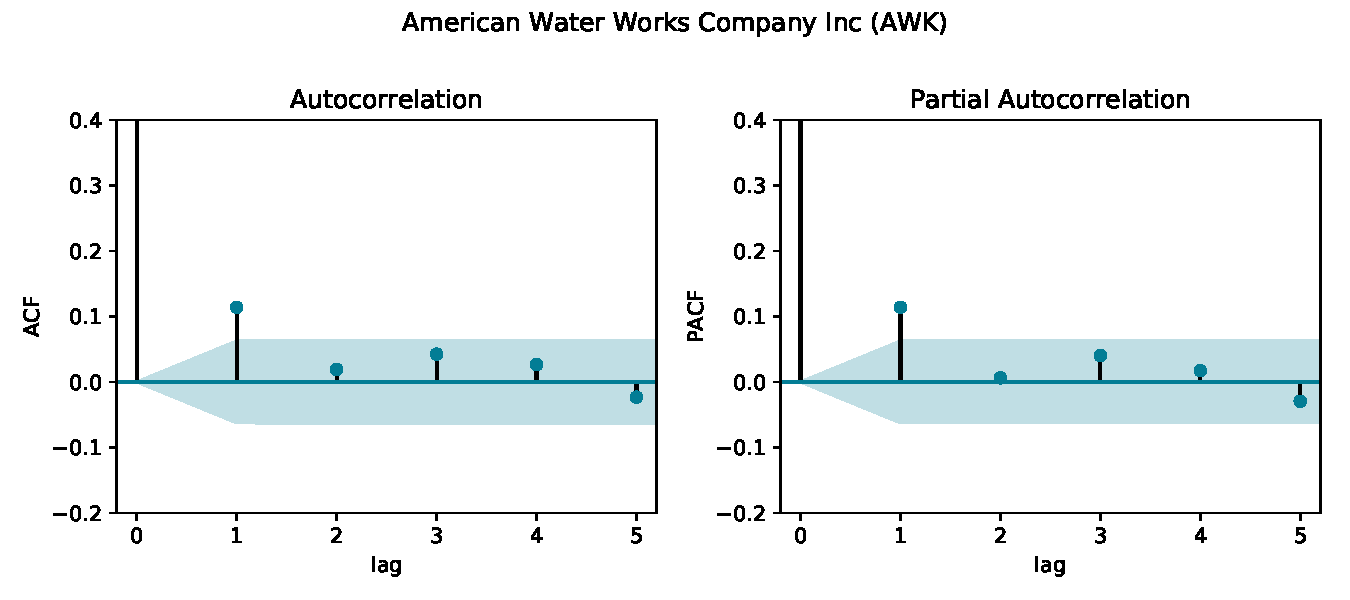
\includegraphics[width=\textwidth]{figures/regression/acf-awk-resid-sqr.pdf}
    \caption{ACF and PACF plot for the squared residuals after applying a ARMA(2, 1) model on the preprocessed stock returns for company \emph{American Water Works Company Inc}.}
    \label{fig:acf_pacf_awk_resid_sqr}
\end{figure}

Figure~\ref{fig:acf_pacf_awk_resid_sqr} visualizes the ACF and PACF for the approximated volatility of an example company by using its squared preprocessed stock returns. The ACF and PACF both reveal significance for the first lag only. This leads to the suggestion of applying a GARCH(1, 1) model.

\begin{figure}[!ht]
    \centering
    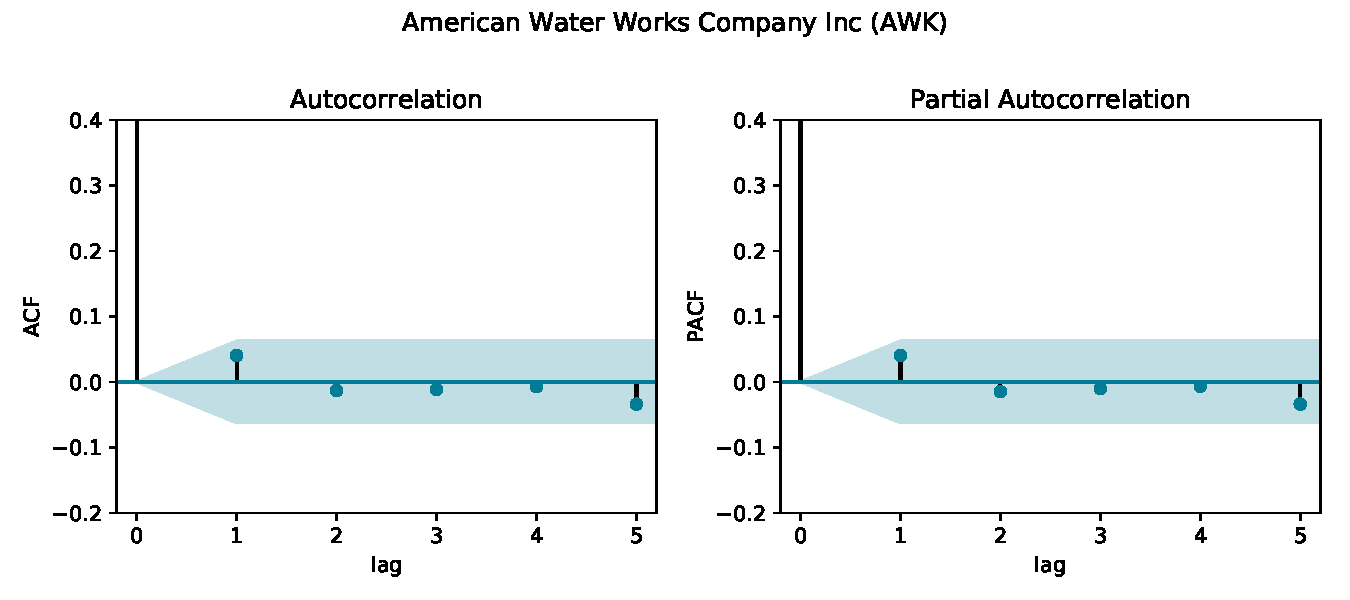
\includegraphics[width=\textwidth]{figures/regression/acf-awk-std-resid-sqr.pdf}
    \caption{ACF plot for the squared residuals after applying a ARMA(2, 1) and a GARCH(1, 1) model on the preprocessed stock returns for company \emph{American Water Works Company Inc}.}
    \label{fig:acf_pacf_awk_std_resid_sqr}
\end{figure}


To evaluate the success of the approach, the ACF and PACF of the standardized residuals are shown in Figure~\ref{fig:acf_pacf_awk_std_resid_sqr}. Clearly, the autocorrelations of the considered lag and even some following lags diminished to a insignificant level close to zero. Under the same procedure, the need of modeling volatility and selection of suitable hyper parameters is examined on all 467 stocks. For 306 from these a GARCH model is applied, usually with $u=1$ and $v=1$.



% The autoregressive–moving-average (ARMA) modelling requires stationarity for calculating its slope coefficients. They are usually calculated using Ordinary Least Squares (OLS) \cite{GrangerNewbold}.


% FORECAST WITH FEASIBLE MODELS: Based on the previously found properties select model (LR, ARIMA, EGARCH, GARCH, etc.). Evaluate models with MAPE (include Diebold and Mariano (DM) test?) and information criterion (AIC, BIC, HCQ). (parametric: ARIMA vs. non-parametric: Link relatives, difference)
%   A) ARIMA parameters can be estimated by finding last significant lag in ACF & PACF. Afterwards evaluate by inspecting "Residual vs fitted" chart and ACF of the models residuals https://newonlinecourses.science.psu.edu/stat510/node/47/
%   B) For predictions: persistence model as baseline

% \subsubsection{Exogeneous Variables}
% Taking GSPC & industry into account as exogeneous variables enables us to reflect other external influences which have an impace on the whole market.